% !TeX spellcheck = en_GB
\chapter{Load balancing}

When dealing with redundant distributed systems, there exists more than one node capable of doing some work.
In such a system the workload needs to be distributed and balanced across all nodes.
This is done using a load balancer with a node balancing algorithm and some performance optimising features.
A node balancer is a service witch distributes incoming requests, among the services registered on the network.
The distribution is based on different policies like dividing packages or picking the one with most free CPU capacity.
The load balancer could be a single point of failure and there should therefore always be more than one as seen in \cref{fig:loadBalancingSetup}.
The load balancer monitors the real servers and only parses on requests to running servers.
A secondary needs to monitor the primary load balancer and step in if it stops responding. This can be done using a virtual private IP, which is the address for all incoming requests.

\begin{figure}
	\centering	
	\scalebox{0.7}{\begin{tikzpicture}[
	start chain=going right,
	diagram item/.style={
		minimum width=80pt,
%		minimum height=45pt,
		on chain,
		join
	},
	diagram item seperated/.style={
			minimum width=80pt,
	%		minimum height=45pt,
			on chain
		}
]
\node [
	diagram item,
  label=center:Internet
] (Internet) {
\includegraphics{Cisco_BW/cloud}};

%\node [
%	continue chain=going below,
%	diagram item,
%	label=right:Router
%] {
\includegraphics{Cisco_BW/router}};

\node [
	start branch=1 going below right,
	diagram item seperated,
	label={[align=center]right:Load\\Balancer\\(Secondary)}
] (LB2) {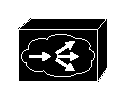
\includegraphics{Cisco_BW/distributed_director}};

\node [
	continue chain=going below left,
	diagram item,
	label={[align=center]left:Load\\Balancer\\(Primary)}
] (LB1) {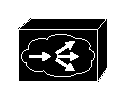
\includegraphics{Cisco_BW/distributed_director}};

\node [
	continue chain = going below right,
	diagram item,
	label={[align=center]right:Services in distrinbuted\\across the wind farm}
] (farm) {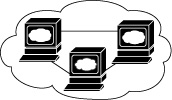
\includegraphics{Cisco_BW/web_cluster}};

\draw[loosely dotted] (LB1) -> (LB2) node[fill=white,midway]{heatbeat};
\draw[dashed] (Internet) -> (LB2);
\draw[dashed] (LB2) -> (farm);

\node [
	start branch=1 going below right,
	diagram item,
	label=below:Other interface
] {\includegraphics{Cisco_BW/PC}};

\node [
	start branch=1 going below left,
	diagram item,
	label=below:Http interface
] {\includegraphics{Cisco_BW/PC}};

\node [
	continue chain = going below,
	diagram item,
	label=below:Modbus interface
] {\includegraphics{Cisco_BW/PC}};

\end{tikzpicture}}
	\captionsetup{format=plain,font=footnotesize,labelfont={bf,defaultCapFont},labelsep=quad,singlelinecheck=no}
	\caption[Distributed System with 2 load balancing nodes]{
		\label{fig:loadBalancingSetup} 
		\footnotesize{%
			A Distributed System with 2 load balancing nodes.
		}
	}
\end{figure}

In this solution the load balancer needs to balance external connections to different protocols like HTTP and Modbus, however a solution witch can be extended to any restful protocol is needed.
Also balancing of node roles depending on the amount incoming traffic on different interfaces will be needed.
Load balancers can also provide features like bundling requests, authentication, discovering bad nodes and caching, all of this offloads the servers behind.

\paragraph{The following requirements to the system exists}
\begin{itemize}
	\item Robustness
	\item Protocol flexible
	\item Must be a distributed component
\end{itemize}

\paragraph{Preferred features}
\begin{itemize}
	\item support TCP Handoffs (for non restful applications)
\end{itemize}

\section{Levels of balancing}
\begin{description}
	\item[OSI 3] Network/IP %google says network layer LVS says transport layer
	\item[OSI 4] Network/IP
	\item[OSI 7] {Application level, like http balancing, allows balancing strategies based on url and user location.}
\end{description}

What we would like is a transport layer protocol.
\cite{Ludwig:SwarmIntelligenceGridLoadBalancing} Implements a particle swam based algorithm, and discuses quality parameters.

\section{Existing solutions}
\begin{description}
	\item[Linux Virtual Server: IPVS] Is implemented in the linux kernal version 2.4 and 2.6. Works at the IP level. Useed byt big sites sourceforge.net, layer 3.
	\item[Google Compute Engine: Load Balancer]: Proprietary. layer 3 and 7.
\end{description}